\documentclass{article}
\usepackage{amsmath, amssymb, amsfonts, amsthm}
\usepackage{tikz}
\usepackage{xcolor}

\newcommand{\Rmax}{R_0^{\text{max}}}
\newcommand{\mmax}[1]{m_{-q}\left(R_0^{\text{max}}, 1\right)}
\newcommand{\gammaq}{\gamma/g_q}

\begin{document}

\begin{figure}[h]
    \centering
    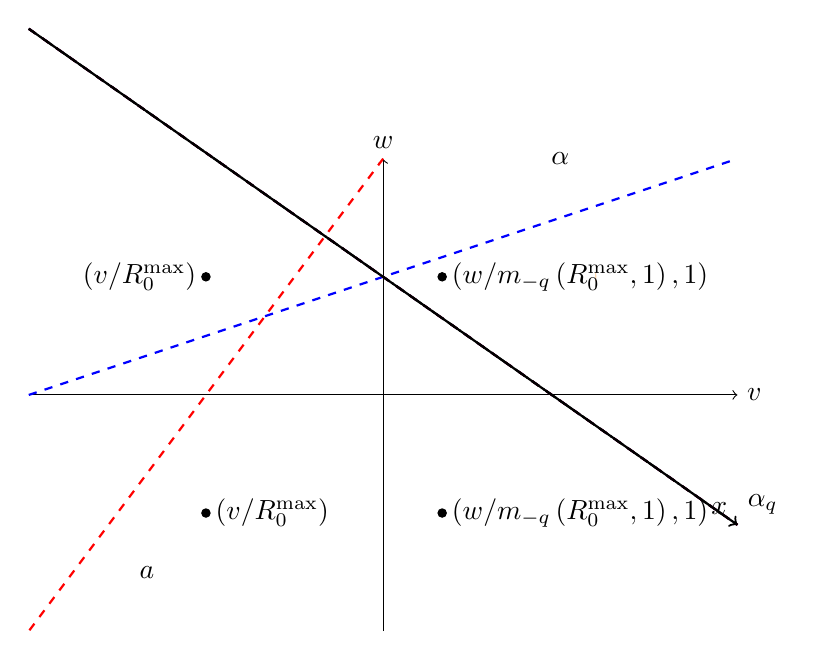
\begin{tikzpicture}[scale=1.5]
        
        % Axes
        \draw[->] (-3,0) -- (3,0) node[right] {$v$};
        \draw[->] (0,-2) -- (0,2) node[above] {$w$};
        
        % Orange Area
        \filldraw[orange!30] plot [smooth cycle,domain=-2:2] ({cos(\x)+0.8},{sin(\x)+1}) node[right] {};
        
        % Dashed Line Supporting K at v
        \draw[dashed, color=blue, thick] (-3,0) -- (3,2);
        \node at (1.5, 2) {$\alpha$};
        
        % Dashed Line Supporting L at w
        \draw[dashed, color=red, thick] (0,2) -- (-3,-2);
        \node at (-2, -1.5) {$a$};
        
        % Dashdotted Line Parallel to Red Line
        \draw[dashdotted, color=black, thick, domain=-3:3] plot (\x,-0.7*\x+1) node [above right] {$\alpha_q$};
        
        % Labels for Points
        \filldraw[black] (-1.5, 1) circle (1pt) node[left] {$(v/\Rmax)$};
        \filldraw[black] (0.5, 1) circle (1pt) node [right] {$(w/\mmax{1},1)$};
        \filldraw[black] (-1.5, -1) circle (1pt) node[right] {$(v/\Rmax)$};
        \filldraw[black] (0.5, -1) circle (1pt) node [right] {$(w/\mmax{1},1)$};
        
        % Ray from v
        \draw[dashed, color=blue, thick, domain=-3:3] plot (\x, -0.7*\x + 1);
        
        % Ray from w
        \draw[dashed, color=red, thick, domain=-3:3] plot (\x, -0.7*\x + 1);
        
        % Line containing x supporting conv(K∪L)
        \draw[thick, domain=-3:3] plot (\x, -0.7*\x + 1) node [above left] {$x$};
        
        % Segment belonging to bd(underline{M}_{q}(K,L))
        \draw[->, dashed, color=black, thick, domain=-3:3] plot (\x, -0.7*\x + 1) node [above right] {};
        
    \end{tikzpicture}
    \caption{Situation in the proof of Lemma~\ref{p-means radii strict inequality lemma}: None of the points on the orange curve (which consists of $\gamma/q$ and two rays) lie in $\inter(K)$, so $K$ is a subset of the orange area. The two dashed lines are parallel and support $K$ at $v$ and $L$ at $w$, respectively. The dashdotted line and segment are also parallel. The line containing $x$ supports $\conv( K \cup L)$ at $x$, whereas the segment belongs to $\bd(\underline{M}_{q}(K,L))$.}
    \label{fig:lemma_diagram}
\end{figure}

\end{document}